%\documentclass[a4paper,handout]{beamer}
\documentclass[presentation]{beamer}
%\usepackage[francais]{babel}
\usepackage[utf8]{inputenc}
\usetheme{Inuits}
\usepackage[T1]{fontenc}
\usepackage{listings}
\usepackage{eso-pic}
\setbeamercolor{background canvas}{bg=} 
\definecolor{inuitstitle}{RGB}{153,153,255}
\definecolor{inuitsgreen}{RGB}{35,255,35}
\usecolortheme[RGB={90,90,149}]{structure} 
\usebackgroundtemplate{%

\includegraphics[height=\paperheight,widht=\paperwidth]{files/background.png};}

%\AddToShipoutPicture{\put(0,5){%
%   \parbox[b][\paperheight]{\paperwidth}{%
%     \vfill
%     \centering
%     \rotatebox{0}{
\includegraphics[width=\paperwidth,height=\paperheight,%
%                      ]{files/background.png}}%
%     \vfill
%}}}
\setbeamercolor{normal text}{fg=white}
\setbeamercolor{block body}{fg=black}
\setbeamercolor{itemize item}{fg=inuitsgreen}
\setbeamercolor{itemize subitem}{fg=inuitsgreen}
\setbeamercolor{itemize subitem subitem}{fg=inuitsgreen}
\setbeamertemplate{itemize item}[circle] 
\setbeamertemplate{itemize subitem}[circle] 
\setbeamertemplate{sections/subsections in toc}[circle]

%\setbeamercolor{palette primary}{fg=inuitstitle,bg=black!85}
%\setbeamercolor{palette secondary}{fg=white,bg=inuitstitle}
%\setbeamercolor{palette tertiary}{fg=white,bg=black!85}
%\setbeamercolor{palette quaternary}{fg=inuitstitle}
%\setbeamercolor{block title}{fg=inuitstitle}
%\setbeamercolor{sidebar}{bg=inuitstitle!70}

%\AtBeginDocument{%
%    \pgfdeclareverticalshading{beamer@topshade}{\paperwidth}{%
%      color(0pt)=(bg);
%      color(4pt)=(black)}
%}


\setbeamercolor{title}{fg=inuitstitle,bg=}

\setbeamertemplate{navigation symbols}{}
\definecolor{OliveGreen}{RGB}{0,100,0}
\definecolor{grey}{RGB}{150,150,150}
\definecolor{darkgrey}{RGB}{100,100,100}
\definecolor{inuits}{RGB}{153,153,255}
\usepackage{shadowtext}
\newcommand{\xitem}[1]{\item{\shadowtext{#1}}}
\newcommand{\inuits}[1]{\shadowtext{\color{inuits}#1}}

\begin{document}
\setbeamercovered{invisible}

\title[Testing your puppet code]{\fontsize{25}{35}\selectfont \shadowtext{Testing your puppet code}}

\author[Julien Pivotto]{\shadowtext{Julien Pivotto}}
%\institute[Inuits]{Inuits}
\date{\shadowtext{Libre Software Meeting 2013}\\\inuits{\today}}
\logo{
\includegraphics[height=1cm]{files/lsm2013.png}}

\frame[plain,t]{\vspace{-1em} \centerline{
\includegraphics[width=\paperwidth]{files/loup.jpg}}\titlepage}
\frame{\tableofcontents}
\section{Introduction}
\frame{%
    \begin{center}\begin{Huge}{\inuits{Julien Pivotto}}\end{Huge}\end{center}
    \begin{large}
    \begin{itemize}
        \xitem{sysadmin @ inuits}
        \xitem{open-source defender for 7+ years}
        \xitem{devops believer}
        \xitem{@roidelapluie on twitter/github}
    \end{itemize}
    \end{large}
}

\subsection{Automation}
\frame{%
\frametitle{Infrastructure as Code}
    \begin{LARGE}
    \begin{itemize}
        \xitem{Keep your environments under SCM}
        \xitem{Overview of complete environments}
        \xitem{Reduce the deployment time}
    \end{itemize}
    \end{LARGE}
}
\frame{%
\frametitle{Keep all environments the same}

    \flushright{\tiny{\color{darkgrey}http://www.flickr.com/photos/bobvietnam/4828291896/}}
    \begin{center}
        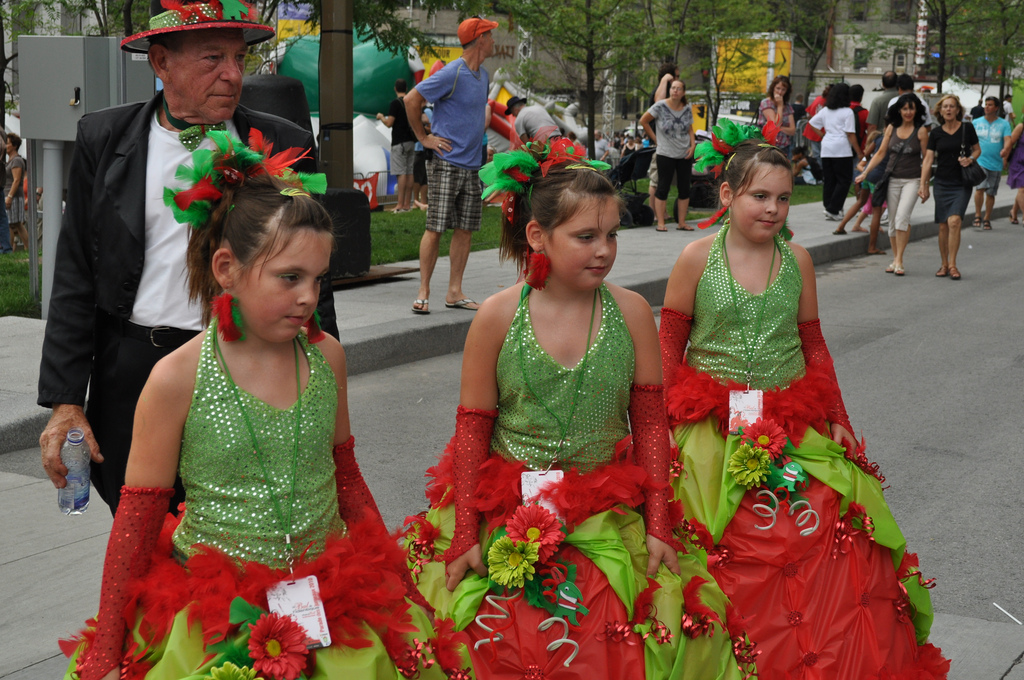
\includegraphics[height=6cm]{files/flickr_jumeaux.jpg}\\
    \end{center}
}
\frame{%
\frametitle{Packaging with FPM}
    \begin{LARGE}
    \begin{itemize}
        \xitem{Ruby gem}
        \xitem{package a directory (and much more)}
        \xitem{Support~.deb,~.rpm}
        \xitem{Package the code with several prefixes}
        \xitem{/etc/puppet/environments/infradev}
        \xitem{/etc/puppet/environments/uat}
    \end{itemize}
    \end{LARGE}
}
\subsection{Vagrant}
\frame{%
\frametitle{Vagrant}
    \begin{LARGE}
    \begin{itemize}
        \xitem{Create virtual machines}
        \xitem{Provision them}
        \xitem{Destroy \& recreate}
    \end{itemize}
    \end{LARGE}
}
\frame{%
\frametitle{Vagrant}
    \begin{LARGE}
    \begin{itemize}
        \xitem{Chef, scripts, puppet, \ldots}
        \xitem{Backend: Virtualbox, KVM, \ldots}
        \xitem{A lot of baseboxes available}
        \xitem{http://vagrantup.com}
    \end{itemize}
    \end{LARGE}
}
\frame{%
\frametitle{Vagrant}
    \begin{LARGE}
    \begin{itemize}
        \xitem{Local testing}
        \xitem{The same environment as the target}
    \end{itemize}
    \end{LARGE}
}
\subsection{Puppet in a large scale}
\frame{%
\frametitle{Puppet environments}
    \begin{large}
    \begin{itemize}
        \xitem{Multiple environments}
        \xitem{The same tree for all the environments}
        \xitem{Pushing changes to UAT/prod on-demand}
        \xitem{Small changes vs big releases}
    \end{itemize}
    \end{large}
}
\frame{%
\frametitle{Hiera}
    \begin{itemize}
        \xitem{Storing the data in Hiera(-gpg)}
        \xitem{Usernames, password, IP addresses}
        \xitem{Hiera is made to be structured}
        \xitem{Using one hiera repo for all the environments}
        \xitem{Using Hiera in your manifests, not in your modules}
    \end{itemize}
}
\frame{%
\frametitle{Hiera tree}
    \begin{LARGE}
    \begin{itemize}
        \xitem{\%\{environment\}/\%\{hostname\}}
        \xitem{\%\{environment\}/common}
        \xitem{infradev/www45.yaml}
        \xitem{infradev/common.yaml}
    \end{itemize}
    \end{LARGE}
}
\subsection{Puppet code}
\frame{%
\frametitle{Keeping clean puppet modules}
    \flushright{\tiny{\color{darkgrey}http://www.flickr.com/photos/aurelie\_solenne/8340968061/}}
    \begin{center}
        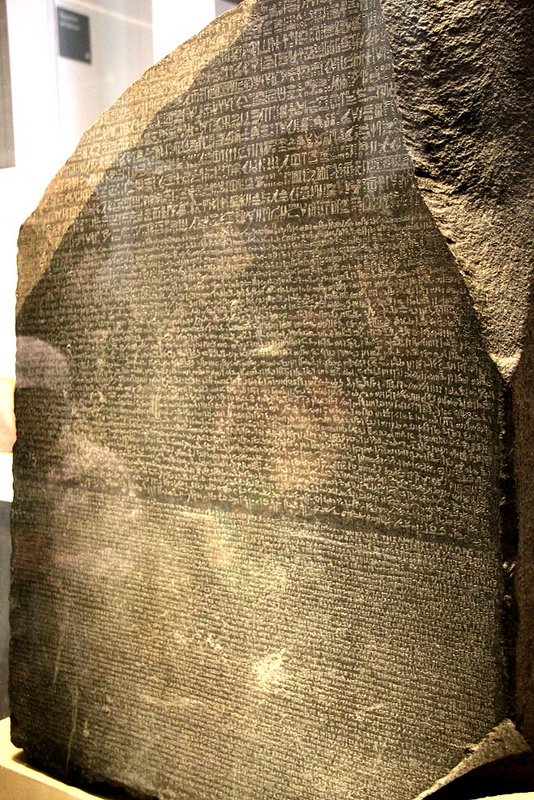
\includegraphics[height=3cm]{files/flickr_rosette.jpg}\\
    \end{center}
    \begin{itemize}
        \xitem{Make them readable}
        \xitem{Make them reusable and sharable}
        \xitem{Don't puppetize everything}
        \xitem{User generated content is not puppetized}
    \end{itemize}
}
\frame{%
\frametitle{Use the right structure for your modules}
    \begin{small}
    \begin{itemize}
        \xitem{Package, config, service}
        \xitem{module::package, module::config, module::service}
        \xitem{Parameterized classes}
    \end{itemize}
    \tiny{\color{inuits}http://www.slideshare.net/PuppetLabs/modern-module-development-ken-barber-2012-edinburgh-puppet-camp}
    \end{small}
}
\frame{%
\frametitle{Distribution-agnostic puppet modules}
    \begin{itemize}
        \xitem{You don't have to support all the distros}
        \xitem{Adding support for another distro should be easy}
    \end{itemize}
    \begin{block}
    \tiny
\texttt{~~\$config\_dir~=~\$configroot~?~\{}\\
\texttt{~~~~undef~~~=>~\$::operatingsystem~?~\{}\\
\texttt{~~~~~~/Debian|Ubuntu/~=>~'/etc/apache2',}\\
\texttt{~~~~~~/CentOS|RedHat/~=>~'/etc/httpd',}\\
\texttt{~~~~~~default~~~~~~~~~=>~'/etc/httpd',}\\
\texttt{~~~~\},}\\
\texttt{~~~~default~=>~\$configroot,}\\
\texttt{~~\}}\\
    \end{block}
}
\frame{%
\frametitle{Puppet function}
    \begin{itemize}
        \xitem{The fail function prevents catalog to be applied}
        \xitem{The notify function prints a warning}
    \end{itemize}
    \begin{block}
    \tiny
\texttt{if~(!\$leftsubnet)~and~(!\$leftsubnets)~\{}\\
\texttt{~fail('\$leftsubnets~and~\$leftsubnet~both~empty')}\\
\texttt{\}}\\
    \end{block}
}
\section{Testing tools}
\subsection{Style and linting}
\frame{%
\frametitle{Puppet parser}
    \begin{itemize}
        \xitem{Included in puppet}
        \xitem{Validating the syntax}
        \xitem{\texttt{puppet parser validate init.pp}}
        \item{\texttt{find~. -name '*.pp' -exec puppet parser validate + ;}}
    \end{itemize}
}
\frame{%
\frametitle{Puppet lint}
    \flushright{\tiny{\color{darkgrey}http://www.flickr.com/photos/voyages-provence/8127668094/}}
    \begin{center}
        
\includegraphics[height=4cm]{files/ecriture.jpg}\\
    \end{center}
    \begin{itemize}
        \xitem{Follow the puppet style guide}
        \xitem{Two-space soft tab}
        \xitem{align fat comma arrows (=>) within blocks of attributes}
        \xitem{http://docs.puppetlabs.com/guides/style\_guide.html}
    \end{itemize}
}
\subsection{Catalogs}
\frame{%
\frametitle{Cucumber puppet}
    \begin{LARGE}
    \begin{itemize}
        \xitem{Write scenarios}
        \xitem{Easy to read (full sentences)}
        \xitem{Use your manifests}
        \xitem{Need some tricks to work with Puppet 3}
        \xitem{Discontinued}
    \end{itemize}
    \end{LARGE}
}
\frame{%
\frametitle{Cucumber example}
\begin{block}{Cucumber}
\tiny
\texttt{Feature:~General~catalog~policy}\\
\texttt{~~In~order~to~ensure~applicability~of~a~host's~catalog}\\
\texttt{~~As~a~manifest~developer}\\
\texttt{~~I~want~all~catalogs~to~obey~some~general~rules}\\
\texttt{}\\
\texttt{~~Scenario~Outline:~Compile~and~verify~catalog}\\
\texttt{~~~~Given~a~node~specified~by~"features/yaml/<hostname>."}\\
\texttt{~~~~When~I~compile~its~catalog}\\
\texttt{~~~~Then~compilation~should~succeed}\\
\texttt{~~~~And~all~resource~dependencies~should~resolve}\\
\texttt{}\\
\texttt{~~~~Examples:}\\
\texttt{~~~~~~|~hostname~~|}\\
\texttt{~~~~~~|~localhost~|}
\end{block}
}

\frame{%
\frametitle{rspec-puppet}
    \begin{large}
    \begin{itemize}
        \xitem{Check what is the behaviour of puppet}
        \xitem{Separate tests per modules}
        \xitem{Add context, facts, \ldots}
        \xitem{Test custom functions, hosts, manifests, \ldots}
    \end{itemize}
    \end{large}
}
\subsection{rspec-puppet}
\frame{%
\frametitle{rspec-puppet}
\begin{block}{Start with rspec puppet}
\tiny
\texttt{gem install rspec-puppet}\\
\texttt{gem install puppet}\\
\texttt{cd my-module}\\
\texttt{rspec-puppet-init}
\end{block}
}
\frame{%
\frametitle{rspec-puppet}
\begin{block}{spec/defines/connection\_spec.rb}
\tiny
\texttt{require~'spec\_helper'}\\
\texttt{describe~'openswan::connection'~do}\\
\texttt{~~describe~'should~require~rightsubnet~or~rightsubnets'~do}\\
\texttt{~~~~let(:title)~\{~'foobar'~\}}\\
\texttt{~~~~let~(:params)~\{~\{}\\
\texttt{~~~~~~:ike~~~~~~~~~=>~'aes256-sha1;modp1024',}\\
\texttt{~~~~~~:esp~~~~~~~~~=>~'aes256-sha1;modp1024',}\\
\texttt{~~~~~~:leftsubnet~=>~'8.8.5.5',}\\
\texttt{~~~~~~:right~~~~~~~=>~'84.54.105.5',}\\
\texttt{~~~~~~:left~~~~~~~~=>~'68.65.98.6',}\\
\texttt{~~~~~~:foreignip~~~=>~'45.25.5.5',}\\
\texttt{~~~~~~:localtestip~=>~'82.8.8.8',~\}~\}}\\
\texttt{~~~~~~it~do}\\
\texttt{~~~~~~~~expect~\{}\\
\texttt{~~~~~~~~~~should~contain\_file("/etc/ipsec.d/foobar.conf")}\\
\texttt{~~~~~~~~\}.to~raise\_error(Puppet::Error,~/\$rightsubnets~and~\$rightsubnet~cannot~be~both~empty/)}\\
\texttt{~~~~~~end}\\
\texttt{~~end}\\
\texttt{end}
\end{block}
}
\frame{%
\frametitle{rspec-puppet}
\begin{block}{Second example}
\tiny
\texttt{require~'spec\_helper'}\\
\texttt{describe~'apache',~:type~=>~:class~do}\\
\texttt{~~let~(:facts)~\{~\{}\\
\texttt{~~~~:operatingsystem~=>~'CentOS',}\\
\texttt{~~~~:osfamily~=>~'RedHat',}\\
\texttt{~~\}~\}}\\
\texttt{~~describe~'without~parameters'~do}\\
\texttt{~~~~it~\{~should~create\_class('apache')~\}}\\
\texttt{~~~~it~\{~should~include\_class('apache::service')~\}}\\
\texttt{~~~~it~\{~should~contain\_apache\_\_listen('80')~\}}\\
\texttt{~~~~it~\{~should~contain\_apache\_\_namevhost('80')~\}}\\
\texttt{~~end}\\
\texttt{end}
\end{block}
}
\frame{%
\frametitle{rspec-puppet}
    \begin{large}
    \begin{itemize}
        \xitem{should, should\_not}
        \xitem{should contain\_package}
        \xitem{contain\_foo\_\_bar('baz') (for foo::bar)}
    \end{itemize}
    \end{large}
}
\section{Jenkins}
\frame{%
\frametitle{Integration with jenkins}
    \begin{LARGE}
    \begin{itemize}
        \xitem{Pulling, testing and deployments}
        \xitem{Push-Test-Package-Deploy}
        \xitem{Continuous integration}
        \xitem{Continuous delivery}
    \end{itemize}
    \end{LARGE}
}
\frame{%
\frametitle{Jenkins pipelines}
    \begin{LARGE}
    \begin{itemize}
        \xitem{Build pipelines}
        \xitem{Overview of what happens}
        \xitem{Getting notified about what failed}
        \xitem{Promoted build plugin}
    \end{itemize}
    \end{LARGE}
}
\frame{%
\frametitle{Jenkins pipelines}
    \begin{center}
        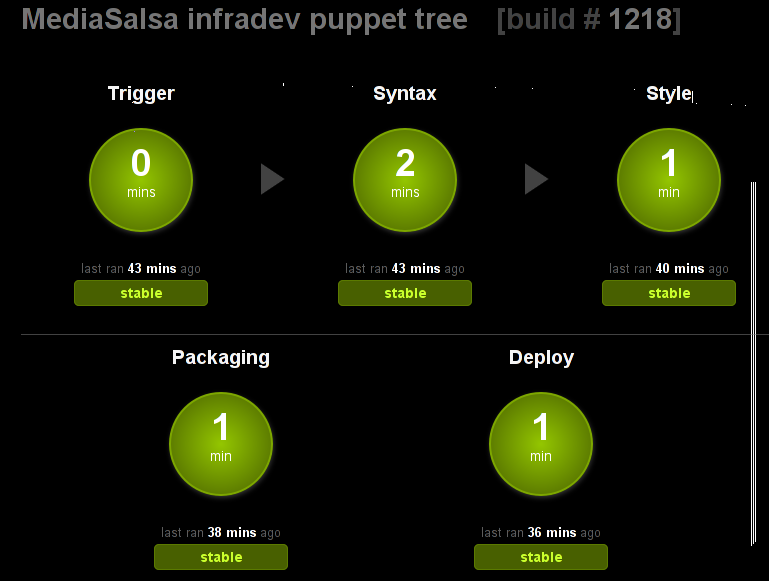
\includegraphics[height=6cm]{files/jenkins1.png}\\
    \end{center}
}
\frame{%
\frametitle{Advantages of CI}
    \begin{center}
        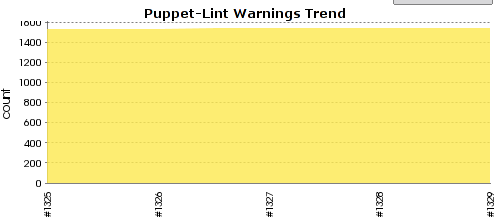
\includegraphics[height=4cm]{files/jenkins2.png}\\
    \end{center}
    \begin{itemize}
        \xitem{You trust your code}
        \xitem{Reproducability}
        \xitem{You get metrics: number of warning, \ldots}
        \xitem{You have a backlog}
        \xitem{It is easy!}
    \end{itemize}
}
\frame{%
\frametitle{Promotions}
    \begin{LARGE}
    \begin{itemize}
        \xitem{Provides buttons you can click}
        \xitem{Trigger actions}
        \xitem{deploy to other environments}
        \xitem{Get a mail with the changes}
        \xitem{Have a log of who deployed}
    \end{itemize}
    \end{LARGE}
}
\frame{%
\frametitle{Promotions}
    \begin{center}
        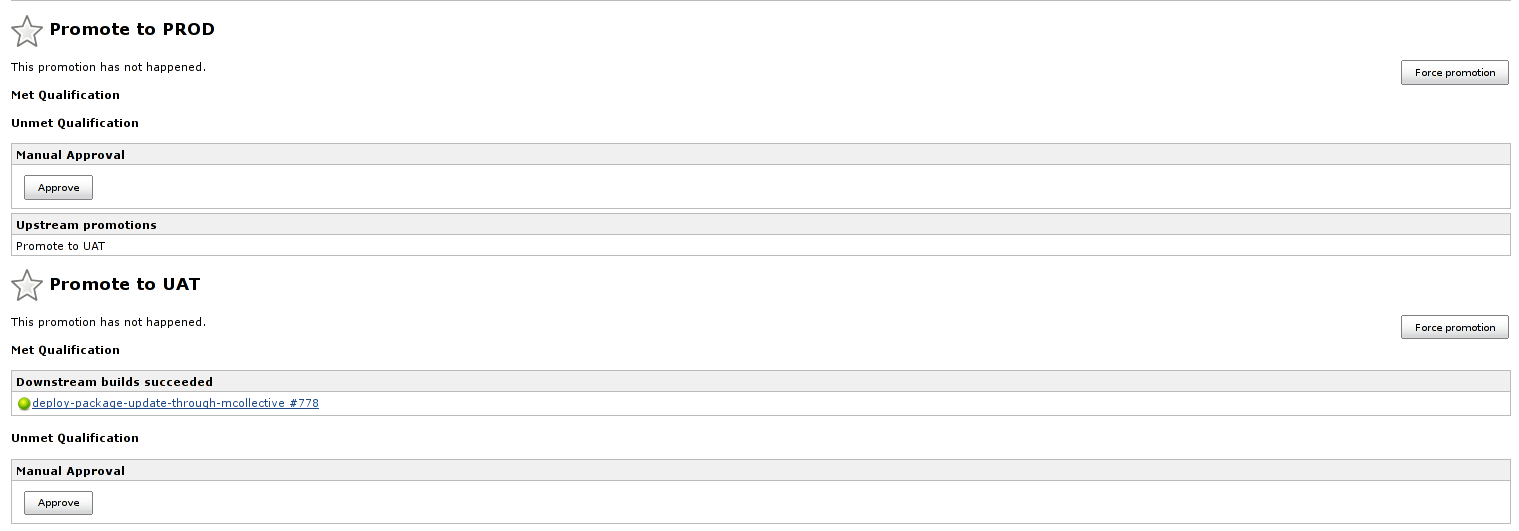
\includegraphics[height=6cm]{files/jenkins3.png}\\
    \end{center}
}
\section{Conclusion}
\subsection{Homework}
\frame{%
\frametitle{Homework}
    \begin{LARGE}
    \begin{itemize}
        \xitem{Integrating tests with git hooks}
        \xitem{Integrating tests with VI}
        \xitem{github.com/philandstuff/fizzgig}
    \end{itemize}
    \end{LARGE}
}
\subsection{Conclusion}
\frame{%
\frametitle{Conclusion}
    \begin{LARGE}
    \begin{itemize}
        \xitem{Use nice \& simple Puppet modules}
        \xitem{Continuous integration}
        \xitem{Multiple environments}
        \xitem{Readability \& reusability}
        \xitem{Tools exist and work together}
    \end{itemize}
    \end{LARGE}
}
\frame{%
\frametitle{Contact}
    \begin{columns}[T]
        \begin{column}{.5\textwidth}
    \begin{large}
    \shadowtext{Julien Pivotto}\\
    \shadowtext{julien@inuits.eu}\\
    \shadowtext{@roidelapluie}
    \end{large}
        \end{column}
        \begin{column}{.5\textwidth}
    \vspace{2cm}
    \begin{small}
    
\includegraphics[height=2cm]{files/inuitslogo.png}\\
    \shadowtext{INUITS bvba}\\
    \shadowtext{Duboisstraat 50}\\
    \shadowtext{2060 Antwerp}\\
    \shadowtext{Belgium}\\
    \shadowtext{+32 473 441 636}\\
    \shadowtext{https://inuits.eu}
    \end{small}
        \end{column}
        \end{columns}
}



\end{document}
